% !TEX TS-program = pdflatex
% !TEX encoding = UTF-8 Unicode

\documentclass[11pt]{report} % use larger type; default would be 10pt

\usepackage[utf8]{inputenc} % set input encoding (not needed with XeLaTeX)

%%% Examples of Article customizations
% These packages are optional, depending whether you want the features they provide.
% See the LaTeX Companion or other references for full information.

%%% PAGE DIMENSIONS
\usepackage{geometry} % to change the page dimensions
\geometry{a4paper} % or letterpaper (US) or a5paper or....
% \geometry{margin=2in} % for example, change the margins to 2 inches all round
% \geometry{landscape} % set up the page for landscape
%   read geometry.pdf for detailed page layout information

\usepackage{graphicx} % support the \includegraphics command and options

% \usepackage[parfill]{parskip} % Activate to begin paragraphs with an empty line rather than an indent

%%% PACKAGES
\usepackage{booktabs} % for much better looking tables
\usepackage{array} % for better arrays (eg matrices) in maths
\usepackage{paralist} % very flexible & customisable lists (eg. itemize/itemize, etc.)
\usepackage{verbatim} % adds environment for commenting out blocks of text & for better verbatim
\usepackage{subfig} % make it possible to include more than one captioned figure/table in a single float
% These packages are all incorporated in the memoir class to one degree or another...

%%% HEADERS & FOOTERS
\usepackage{fancyhdr} % This should be set AFTER setting up the page geometry
\pagestyle{fancy} % options: empty , plain , fancy
\renewcommand{\headrulewidth}{0pt} % customise the layout...
\lhead{}\chead{Links}\rhead{}
\lfoot{}\cfoot{\thepage}\rfoot{}

%%% SECTION TITLE APPEARANCE
\usepackage{sectsty}
\allsectionsfont{\sffamily\mdseries\upshape} % (See the fntguide.pdf for font help)
% (This matches ConTeXt defaults)

%%% ToC (table of contents) APPEARANCE
\usepackage[nottoc,notlof,notlot]{tocbibind} % Put the bibliography in the ToC
\usepackage[titles,subfigure]{tocloft} % Alter the style of the Table of Contents
\renewcommand{\cftsecfont}{\rmfamily\mdseries\upshape}
\renewcommand{\cftsecpagefont}{\rmfamily\mdseries\upshape} % No bold!

%%% END Article customizations

%%% The "real" document content comes below...

\title{Links - Project Proposal}
\author{Abhijith Madhav, Arjun S Bharadwaj}
\date{} % Activate to display a given date or no date (if empty),
         % otherwise the current date is printed 

\begin{document}
\maketitle
\section*{Team Members}
\begin{tabular}{ | c | c | c | }
\hline            
  Name & Role No. & Email id \\
  \hline  
  \hline  
  Abhijith Madhav & MT2013002 & abhijith.madhav@iiitb.org \\
  \hline  
  Arjun S Bharadwaj & MT2013026 & arjun.s.waj@iiitb.org \\  
\hline  
\end{tabular}

\section*{Supervisor}
Prof. Srisha Rao.

\section*{Version}
\begin{tabular}{ | c | c | c | }
\hline            
  Sl. No. & Date. & Version No. \\
\hline  
\hline  
  1 & \date{29/03/2014} & 1 \\
\hline  
\end{tabular}

\section*{Project Timelines}
\begin{itemize}
\item
Start Date: \date{31/01/2014}
\item
End Date: \date{30/06/2014}
\end{itemize}

\section*{Objectives of the project}
Traditional bookmarking services do not allow storing information on private servers. The application should allow deploying a local server which is capable of the following for every user/client:
\begin{itemize}
\item
Bookmarking URLs
\item
Tagging the URLs
\item
Searching among the links
\item
Annotations for a given URL
\item
Multi-user
\item
Expose an API
\end{itemize}

\section*{Functionalities}
This section provides the list of functionalities/features that are planned to be supported in the course of this project.
\begin{itemize}
\item
	Create user accounts/signup.
\item
Links Management
\begin{itemize}
	\item
		Save links.
	\item
		Edit links.
	\item
		Delete links.
	\item
		Tag links.
	\item
		Annotate links.
	\item
		Classify/Organize links in folders.
\end{itemize}
\item
Group Management
\begin{itemize}
	\item
		Create user groups.
	\item
		Join group.
	\item
		Unjoin the group.
	\item
		Add members to the group (by group owner).
	\item
		Remove members from group (by group owner).
\end{itemize}
\item
Share Options
\begin{itemize}
	\item
		Via Email.
	\item
		Via Twitter.
	\item
		Via Facebook.
	\item
		Share links with groups.
\end{itemize}
\item
Suggestions
\begin{itemize}
	\item
		Suggest tags if same link was shared by others if the links privacy is public.
	\item
		Suggest public links belonging to the same tags.
\end{itemize}
\item
Expose APIs
\begin{itemize}
	\item
	Search based on links, annotations, tags at various granularity levels of ownership of the links.
	\item
	APIs to add, delete and edit the links.
	\item
	Android App that consumes the data from the provided APIs.
\end{itemize}
\item
Shorten the links - URL shortener.
\end{itemize}



\section*{Project Deliverables}
This section gives an overview of the deliverables of the project `Links':
\subsection*{Milestones}
The project `Links' shall have the following milestones that shall be delivered.
\begin{itemize}
\item
Freezing on the project requirements through requirement gathering sessions with the client.
\item
Finalization of the Software Requirement Specifications composing both the functional requirements and the non functional requirements.
\item
High level design including the Architecture Design of the core system and the plugin interface.
\item
Low level design including the UML diagrams that conforms to MVC architecture.
\item
Implementataion of the basic and the core functionality of the system.
\item
Implementataion of the plugin architecture to support plugins.
\item
Implementation of the REST APIs.
\item
Implementation of the Android App to consume data through REST APIs.
\item
Unit Testing of the modules.
\end{itemize}

\section*{Estimated total time}
\begin{tabular}{ | c | c | c | }
\hline            
  Sl. No. & Item & Duration (in hours) \\
\hline  
\hline  
  1 & Analysis & 10 \\
\hline  
\hline  
  2 & Requirements Gathering & 10 \\
\hline  
\hline  
  3 & SRS & 15 \\
\hline  
\hline  
  4 & Use Cases & 15 \\
\hline  
\hline  
  5 & High Level Design & 30 \\
\hline  
\hline  
  6 & Low Level Design & 40 \\
\hline  
\hline  
  7 & Implementation & 100 \\
\hline  
\hline  
  8 & Testing & 30 \\
\hline  
\end{tabular}

\section*{H/W and S/W requirements}
This section deals with the H/W and the S/W requirements for the implementation of the project `Links'.
\subsection*{H/W requirements}
The server should have the following configuration:
\begin{itemize}
\item
32/64-bit processor.
\item
At least 2 GB of physical memory.
\item
At least 10 GB of free space.
\end{itemize}

\subsection*{S/W requirements}
The server should have the stable version of the following softwares installed:
\begin{itemize}
\item
Unix based OS.
\item
Ruby.
\item
Rails.
\item
MySQL.
\end{itemize}

\section*{Standards}
The project conforms to the following standards:
\begin{itemize}
\item
Separation of Concerns as laid down by MVC framework.
\item
Conventions over Configurations as laid down by Rails framework.
\item
DRY - Don't Repeat Yourself as laid down by Rails framework.
\item
Mapping resource to the URLs as laid down by REST architecture.
\end{itemize}

\section*{Technology/Architecture}
The project `Links' uses the MVC architecture for the implementation. Below is the architecture diagram of the same.

\begin{figure}[h]
\centering
        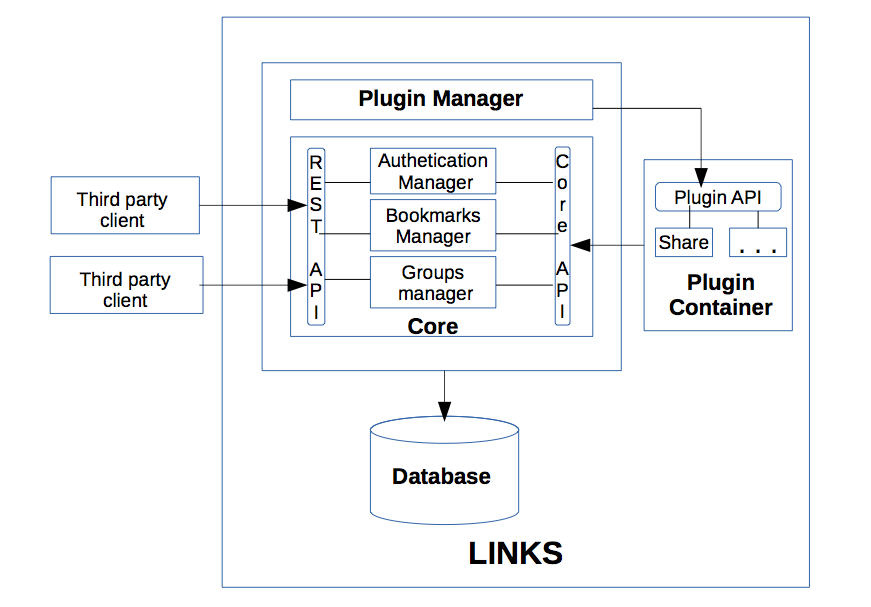
\includegraphics[width=\textwidth]{architecture-diagram}
    \caption{{Links - Architecture Diagram}.}
    \label{fig:Architecture Diagram}
\end{figure}



\end{document}
